% Options for packages loaded elsewhere
\PassOptionsToPackage{unicode}{hyperref}
\PassOptionsToPackage{hyphens}{url}
%
\documentclass[
  english,
  man]{apa6}
\usepackage{lmodern}
\usepackage{amssymb,amsmath}
\usepackage{ifxetex,ifluatex}
\ifnum 0\ifxetex 1\fi\ifluatex 1\fi=0 % if pdftex
  \usepackage[T1]{fontenc}
  \usepackage[utf8]{inputenc}
  \usepackage{textcomp} % provide euro and other symbols
\else % if luatex or xetex
  \usepackage{unicode-math}
  \defaultfontfeatures{Scale=MatchLowercase}
  \defaultfontfeatures[\rmfamily]{Ligatures=TeX,Scale=1}
\fi
% Use upquote if available, for straight quotes in verbatim environments
\IfFileExists{upquote.sty}{\usepackage{upquote}}{}
\IfFileExists{microtype.sty}{% use microtype if available
  \usepackage[]{microtype}
  \UseMicrotypeSet[protrusion]{basicmath} % disable protrusion for tt fonts
}{}
\makeatletter
\@ifundefined{KOMAClassName}{% if non-KOMA class
  \IfFileExists{parskip.sty}{%
    \usepackage{parskip}
  }{% else
    \setlength{\parindent}{0pt}
    \setlength{\parskip}{6pt plus 2pt minus 1pt}}
}{% if KOMA class
  \KOMAoptions{parskip=half}}
\makeatother
\usepackage{xcolor}
\IfFileExists{xurl.sty}{\usepackage{xurl}}{} % add URL line breaks if available
\IfFileExists{bookmark.sty}{\usepackage{bookmark}}{\usepackage{hyperref}}
\hypersetup{
  pdftitle={How to use papaja: An Example Manuscript Including Basic Instructions},
  pdfauthor={Cengiz ZopluogluUniversity of Oregon},
  pdflang={en-EN},
  hidelinks,
  pdfcreator={LaTeX via pandoc}}
\urlstyle{same} % disable monospaced font for URLs
\usepackage{graphicx,grffile}
\makeatletter
\def\maxwidth{\ifdim\Gin@nat@width>\linewidth\linewidth\else\Gin@nat@width\fi}
\def\maxheight{\ifdim\Gin@nat@height>\textheight\textheight\else\Gin@nat@height\fi}
\makeatother
% Scale images if necessary, so that they will not overflow the page
% margins by default, and it is still possible to overwrite the defaults
% using explicit options in \includegraphics[width, height, ...]{}
\setkeys{Gin}{width=\maxwidth,height=\maxheight,keepaspectratio}
% Set default figure placement to htbp
\makeatletter
\def\fps@figure{htbp}
\makeatother
\setlength{\emergencystretch}{3em} % prevent overfull lines
\providecommand{\tightlist}{%
  \setlength{\itemsep}{0pt}\setlength{\parskip}{0pt}}
\setcounter{secnumdepth}{-\maxdimen} % remove section numbering
% Make \paragraph and \subparagraph free-standing
\ifx\paragraph\undefined\else
  \let\oldparagraph\paragraph
  \renewcommand{\paragraph}[1]{\oldparagraph{#1}\mbox{}}
\fi
\ifx\subparagraph\undefined\else
  \let\oldsubparagraph\subparagraph
  \renewcommand{\subparagraph}[1]{\oldsubparagraph{#1}\mbox{}}
\fi
% Manuscript styling
\usepackage{upgreek}
\captionsetup{font=singlespacing,justification=justified}

% Table formatting
\usepackage{longtable}
\usepackage{lscape}
% \usepackage[counterclockwise]{rotating}   % Landscape page setup for large tables
\usepackage{multirow}		% Table styling
\usepackage{tabularx}		% Control Column width
\usepackage[flushleft]{threeparttable}	% Allows for three part tables with a specified notes section
\usepackage{threeparttablex}            % Lets threeparttable work with longtable

% Create new environments so endfloat can handle them
% \newenvironment{ltable}
%   {\begin{landscape}\begin{center}\begin{threeparttable}}
%   {\end{threeparttable}\end{center}\end{landscape}}
\newenvironment{lltable}{\begin{landscape}\begin{center}\begin{ThreePartTable}}{\end{ThreePartTable}\end{center}\end{landscape}}

% Enables adjusting longtable caption width to table width
% Solution found at http://golatex.de/longtable-mit-caption-so-breit-wie-die-tabelle-t15767.html
\makeatletter
\newcommand\LastLTentrywidth{1em}
\newlength\longtablewidth
\setlength{\longtablewidth}{1in}
\newcommand{\getlongtablewidth}{\begingroup \ifcsname LT@\roman{LT@tables}\endcsname \global\longtablewidth=0pt \renewcommand{\LT@entry}[2]{\global\advance\longtablewidth by ##2\relax\gdef\LastLTentrywidth{##2}}\@nameuse{LT@\roman{LT@tables}} \fi \endgroup}

% \setlength{\parindent}{0.5in}
% \setlength{\parskip}{0pt plus 0pt minus 0pt}

% \usepackage{etoolbox}
\makeatletter
\patchcmd{\HyOrg@maketitle}
  {\section{\normalfont\normalsize\abstractname}}
  {\section*{\normalfont\normalsize\abstractname}}
  {}{\typeout{Failed to patch abstract.}}
\patchcmd{\HyOrg@maketitle}
  {\section{\protect\normalfont{\@title}}}
  {\section*{\protect\normalfont{\@title}}}
  {}{\typeout{Failed to patch title.}}
\makeatother
\shorttitle{SHORTTITLE}
\usepackage{csquotes}
\ifxetex
  % Load polyglossia as late as possible: uses bidi with RTL langages (e.g. Hebrew, Arabic)
  \usepackage{polyglossia}
  \setmainlanguage[]{english}
\else
  \usepackage[shorthands=off,main=english]{babel}
\fi

\title{How to use papaja: An Example Manuscript Including Basic Instructions}
\author{Cengiz Zopluoglu\textsuperscript{University of Oregon}}
\date{2020-11-30}


\affiliation{\phantom{0}}

\abstract{
This manuscript demonstrates how to use R Markdown and papaja to create an APA conform manuscript. papaja builds on R Markdown, which uses pandoc to turn Markdown into PDF or Word documents. The conversion to Word documents currently supports only a limited set of features.
}



\begin{document}
\maketitle

\hypertarget{what-is-papaja}{%
\section{What is papaja?}\label{what-is-papaja}}

Reproducible data analysis is an easy to implement and important aspect of the strive towards reproducibility in science.
For \emph{R} users, R Markdown has been suggested as one possible framework for reproducible analyses.
\texttt{papaja} is a R-package in the making including a \href{http://rmarkdown.rstudio.com/}{R Markdown} template that can be used with (or without) \href{http://www.rstudio.com/}{RStudio} to produce documents, which conform to the American Psychological Association (APA) manuscript guidelines (6th Edition).
The package uses the \LaTeX document class \href{http://www.ctan.org/pkg/apa6}{apa6} and a .docx-reference file, so you can create PDF documents, or Word documents if you have to.
Moreover, \texttt{papaja} supplies R-functions that facilitate reporting results of your analyses in accordance with APA guidelines.

Markdown is a simple formatting syntax that can be used to author HTML, PDF, and MS Word documents (among others).
In the following I will assume you know how to use R Markdown to conduct and comment your analyses.
If this is not the case, I recommend you familiarize yourself with \href{http://rmarkdown.rstudio.com/}{R Markdown} first.
I use \href{http://www.rstudio.com/}{RStudio} to create my documents, but the general process works with any text editor.

\hypertarget{how-to-use-papaja}{%
\section{How to use papaja}\label{how-to-use-papaja}}

Once you have installed \texttt{papaja} and all other \href{https://github.com/crsh/papaja\#requirements}{required software}, you can select the APA template when creating a new R Markdown file through the RStudio menus, see Figure~\ref{fig:rstudio}.
When you click RStudio's \emph{Knit} button, \texttt{papaja}, \texttt{bookdown}, \texttt{rmarkdown,} and \texttt{knitr} work together to create an APA conform manuscript that includes both your text and the output of any embedded R code chunks within the manuscript.

If you don't use RStudio, you can create new \texttt{papaja} documents via \texttt{rmarkdown::draft()} and \texttt{rmarkdown::render()}.

\hypertarget{printing-r-output}{%
\subsection{Printing R output}\label{printing-r-output}}

Any output from R is included as you usually would using R Markdown.
By default the R code will not be displayed in the final documents.
If you wish to show off your code you need to set \texttt{echo\ =\ TRUE} in the chunk options.
For example, to include summary statistics of your data you could use the following code:

\begin{verbatim}
##       sid          reading            ses            race     
##  Min.   :1002   Min.   : 33.14   Min.   :-2.33000   A  :1259  
##  1st Qu.:1342   1st Qu.: 46.73   1st Qu.:-0.66500   AI : 338  
##  Median :1678   Median : 53.03   Median :-0.13900   B  :2295  
##  Mean   :1672   Mean   : 54.44   Mean   :-0.04386   H  :2930  
##  3rd Qu.:2006   3rd Qu.: 58.94   3rd Qu.: 0.53500   HPI: 173  
##  Max.   :2330   Max.   :164.33   Max.   : 2.59600   W  :7074
\end{verbatim}

But, surely, this is not what you want your submission to look like.

\hypertarget{print-tables}{%
\subsubsection{Print tables}\label{print-tables}}

For prettier tables, I suggest you try \texttt{apa\_table()}, which builds on \texttt{knitr}'s \texttt{kable()}, and \texttt{printnum()}, which can be used to properly round and report numbers.
For the table to display correctly set the chunk option \texttt{results\ =\ "asis"} in the chunk that produces the table.

\begin{table}[tbp]

\begin{center}
\begin{threeparttable}

\caption{\label{tab:unnamed-chunk-2}Descriptive statistics of reading scores by race}

\begin{tabular}{lllll}
\toprule
race & \multicolumn{1}{c}{Mean} & \multicolumn{1}{c}{SD} & \multicolumn{1}{c}{Min} & \multicolumn{1}{c}{Max}\\
\midrule
A & 60.65 & 16.14 & 33.71 & 115.04\\
AI & 51.29 & 9.68 & 33.78 & 102.66\\
B & 52.63 & 10.37 & 33.41 & 113.45\\
H & 50.44 & 9.68 & 33.14 & 107.71\\
HPI & 54.58 & 12.52 & 34.30 & 104.81\\
W & 55.72 & 11.20 & 33.22 & 164.33\\
\bottomrule
\addlinespace
\end{tabular}

\begin{tablenotes}[para]
\normalsize{\textit{Note.} This table was created with apa\_table()}
\end{tablenotes}

\end{threeparttable}
\end{center}

\end{table}

Of course popular packages like \texttt{xtable}\footnote{When you use \texttt{xtable()}, table captions are \href{http://tex.stackexchange.com/questions/42209/centering-tables-in-document-class-apa6}{set to the left page margin}.} or \texttt{tables} can also be used to create tables when knitting PDF documents.
These packages, however, cannot be used when you want to create Microsoft Word documents because they rely on \LaTeX for typesetting.
\texttt{apa\_table()} creates tables that conform to APA guidelines and are correctly rendered in PDF and Word documents.
But don't get too excited; table formatting is somewhat limited for Word documents due to missing functionality in pandoc (e.g., it is not possible to have cells or headers span across multiple columns).

As required by the APA guidelines, tables are deferred to the final pages of the manuscript when creating a PDF.
Again, this is not the case in Word documents due to limited pandoc functionality.
To place tables and figures in your text instead, set the \texttt{figsintext} parameter in the YAML header to \texttt{yes} or \texttt{true}, as I have done in this document.

The bottom line is, Word documents will be less polished than PDF.
The resulting documents should suffice to enable collaboration with Wordy colleagues and prepare a journal submission with limited manual labor.

\hypertarget{embed-plots}{%
\subsubsection{Embed plots}\label{embed-plots}}

As usual in R Markdown, you can embed R-generated plots into your document, see Figure~\ref{fig:beeplot}.

\textbackslash begin\{figure\}

\{\centering 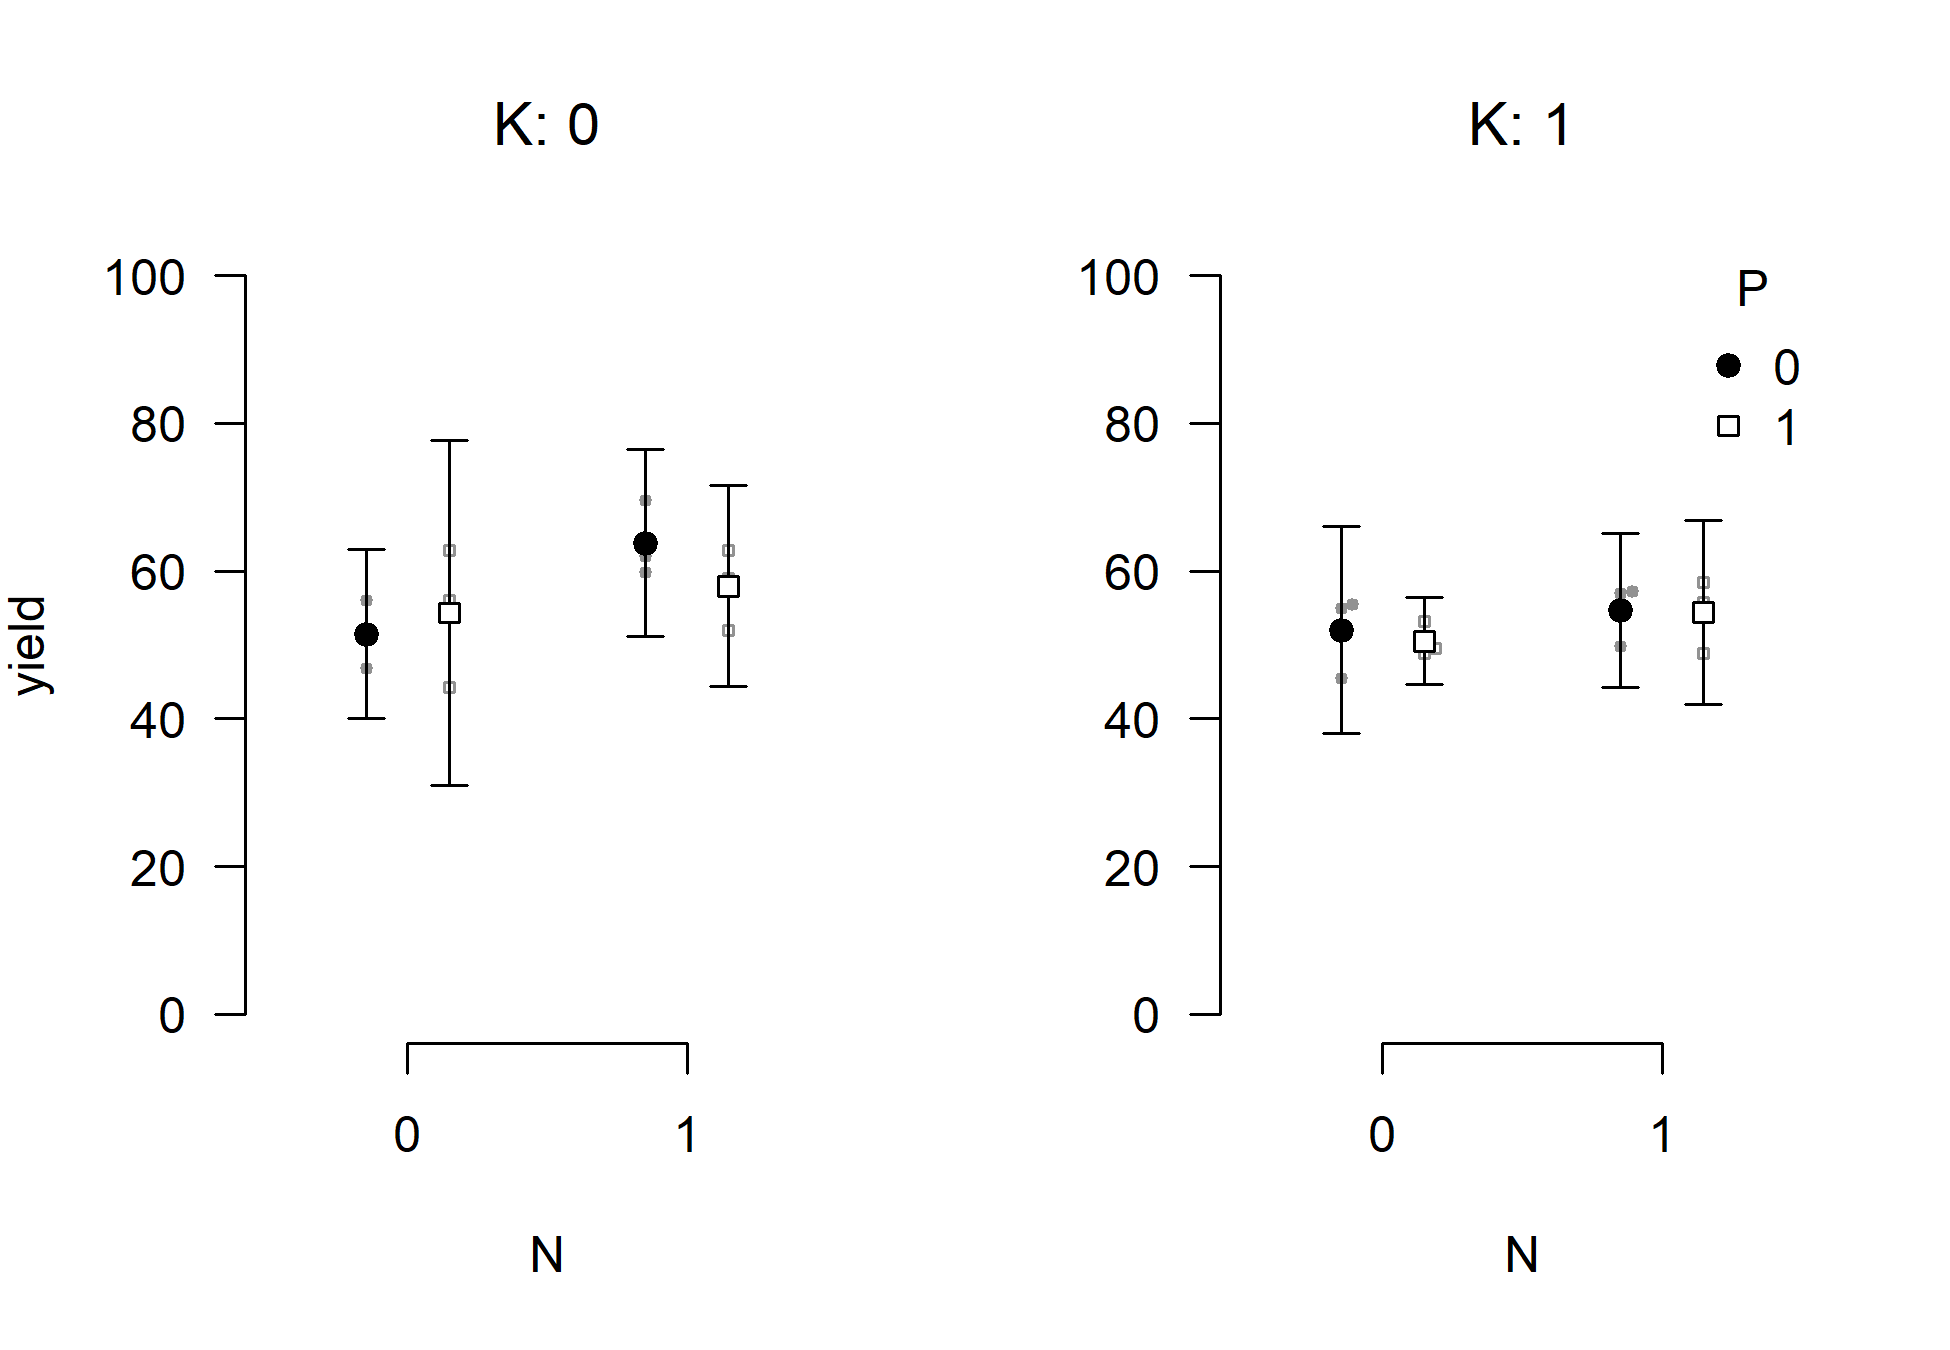
\includegraphics{template_files/figure-latex/beeplot-1}

\}

\textbackslash caption\{Bee plot of the example data set. Small points represent individual observations, large points represent means, and error bars represent 95\% confidence intervals.\}\label{fig:beeplot}
\textbackslash end\{figure\}

Again, as required by the APA guidelines, figures are deferred to the final pages of the document unless you set \texttt{figsintext} to \texttt{yes}.

\hypertarget{referencing-figures-and-tables}{%
\subsubsection{Referencing figures and tables}\label{referencing-figures-and-tables}}

\texttt{papaja} builds on the \texttt{bookdown} package, which provides limited cross-referencing capabilities within documents.
By default you can insert figure and table numbers into the text using \texttt{\textbackslash{}@ref(fig:chunk-name)} for figures or \texttt{\textbackslash{}@ref(tab:chunk-name)} for tables.
Note that for this syntax to work chunk names cannot include \texttt{\_}.
If you need to embed an external image that is not generated by R use the \texttt{knitr::include\_graphics()} function.
See the \href{https://bookdown.org/yihui/bookdown/cross-references.html}{great book on \texttt{bookdown}} for details.
Cross-referencing is currently not available for equations in \texttt{bookdown}.
However, as anywhere in R Markdown documents you can use \LaTeX commands if the functionality is not provided by \texttt{rmarkdown}/\texttt{bookdown} and you don't need to create Word documents.

\hypertarget{report-statistical-analyses}{%
\subsubsection{Report statistical analyses}\label{report-statistical-analyses}}

\texttt{apa\_print()} will help you report the results of your statistical analyses.
The function will format the contents of R objects and produce readily reportable text.

Now, you can report the results of your analyses like so:

Race is related to reading scores after accounting for SES,
\(F(5, 14,063) = 184.91\), \(\mathit{MSE} = 127.63\), \(p < .001\), \(\hat{\eta}^2_p = .062\).

What's even more fun, you can easily create a complete ANOVA table using by passing \texttt{mod\_results\$table} to \texttt{apa\_table()}, see Table~\ref{tab:anova-table}.

\begin{table}[tbp]

\begin{center}
\begin{threeparttable}

\caption{\label{tab:anova-table}ANOVA table for the analyis of the example data set.}

\begin{tabular}{lrcrrrl}
\toprule
Effect & \multicolumn{1}{c}{$F$} & \multicolumn{1}{c}{$\mathit{df}_1$} & \multicolumn{1}{c}{$\mathit{df}_2$} & \multicolumn{1}{c}{$\mathit{MSE}$} & \multicolumn{1}{c}{$p$} & \multicolumn{1}{c}{$\hat{\eta}^2_p$}\\
\midrule
Race & 184.91 & 5 & 14,063 & 127.63 & < .001 & .062\\
\bottomrule
\addlinespace
\end{tabular}

\begin{tablenotes}[para]
\normalsize{\textit{Note.} This is a table created using apa\_print() and apa\_table().}
\end{tablenotes}

\end{threeparttable}
\end{center}

\end{table}

\hypertarget{citations}{%
\subsection{Citations}\label{citations}}

No manuscript is complete without citation.
In order for citations to work, you need to supply a .bib-file to the \texttt{bibliography} parameter in the YAML front matter.
Once this is done, \texttt{{[}e.g.,\ @james\_1890;\ @bem\_2011{]}} produces a regular citation within parentheses (e.g., Bem, 2011; James, 1890).
To cite a source in text simply omit the brackets; for example, write \texttt{@james\_1890} to cite James (1890).
For other options see the \href{http://rmarkdown.rstudio.com/authoring_bibliographies_and_citations.html}{overview of the R Markdown citation syntax}.

The citation style is automatically set to APA style.
If you need to use a different citation style, you can set in the YAML front matter by providing the \texttt{csl} parameter.
See the \href{http://R\%20Markdown.rstudio.com/authoring_bibliographies_and_citations.html}{R Markdown documentation} and \href{http://citationstyles.org/}{Citation Style Language} for further details.

If you use RStudio, I have created an \href{https://github.com/crsh/citr}{easy-to-use add-in} that facilitates inserting citations into a document.
The relevant references will, of course, be added to the documents reference section automatically.
Moreover, the addin can directly access you Zotero database.

I think it is important to credit the software we use.
A lot of R packages are developed by academics free of charge.
As citations are the currency of science, it's easy to compensate volunteers for their work by citing the R packages we use.
I suspect that, among other things, this is rarely done because it is tedious work.
That's why papaja makes citing R and its packages easy:

\texttt{r\_refs()} creates a BibTeX file containing citations for R and all currently loaded packages.
\texttt{cite\_r()} takes these citations and turns them into readily reportable text.
\texttt{my\_citation} now contains the following text that you can use in your document: R (Version 4.0.2; R Core Team, 2020) and the R-packages \emph{afex} (Version 0.28.0; Singmann, Bolker, Westfall, Aust, \& Ben-Shachar, 2020), \emph{dplyr} (Version 1.0.2; Wickham, François, Henry, \& Müller, 2020), \emph{lme4} (Version 1.1.23; Bates, Mächler, Bolker, \& Walker, 2015), \emph{Matrix} (Version 1.2.18; Bates \& Maechler, 2019), and \emph{papaja} (Version 0.1.0.9997; Aust \& Barth, 2020)

\hypertarget{math}{%
\subsection{Math}\label{math}}

If you need to report formulas, you can use the flexible \LaTeX syntax (it will work in Word documents, too).
Inline math must be enclosed in \texttt{\$} or \texttt{\textbackslash{}(} and \texttt{\textbackslash{})} and the result will look like this: \(d' = z(H) - z(FA)\).
For larger formulas displayed equations are more appropriate; they are enclosed in \texttt{\$\$} or \texttt{\textbackslash{}{[}}and \texttt{\textbackslash{}{]}},

\[
d' = \frac{\mu_{old} - \mu_{new}}{\sqrt{0.5(\sigma^2_{old} + \sigma^2_{new})}}.
\]

\hypertarget{document-options}{%
\subsection{Document options}\label{document-options}}

This text is set as manuscript.
If you want a thesis-like document you can change the \texttt{class} in the YAML front matter from \texttt{man} to \texttt{doc}.
You can also preview a polished journal typesetting by changing the \texttt{class} to \texttt{jou}.
Refer to the \texttt{apa6} document class \href{ftp://ftp.fu-berlin.de/tex/CTAN/macros/latex/contrib/apa6/apa6.pdf}{documentation} for further \texttt{class} options, such as paper size or draft watermarks.

When creating PDF documents, line numbering can be activated by setting the \texttt{lineno} argument in the YAML front matter to \texttt{yes}.
Moreover, you can create lists of figure or table captions at the end of the document by setting \texttt{figurelist} or \texttt{tablelist} to \texttt{yes}, respectively.
These option have no effect on Word documents.

\hypertarget{last-words}{%
\subsection{Last words}\label{last-words}}

That's all I have; enjoy writing your manuscript.
If you have any trouble or ideas for improvements, open an \href{https://github.com/crsh/papaja/issues}{issue} on GitHub or open a pull request.
If you want to contribute, take a look at the \href{https://github.com/crsh/papaja/issues}{open issues} if you need inspiration.
Other than that, there are many output objects from analysis methods that we would like \texttt{apa\_print()} to support.
Any new S3/S4-method for this function are always appreciated (e.g., \texttt{factanal}, \texttt{fa}, \texttt{lavaan}, \texttt{BFBayesFactor}).

\hypertarget{references}{%
\section{References}\label{references}}

\setlength{\parindent}{-0.5in}
\setlength{\leftskip}{0.5in}

\hypertarget{refs}{}
\leavevmode\hypertarget{ref-R-papaja}{}%
Aust, F., \& Barth, M. (2020). \emph{papaja: Create APA manuscripts with R Markdown}. Retrieved from \url{https://github.com/crsh/papaja}

\leavevmode\hypertarget{ref-R-Matrix}{}%
Bates, D., \& Maechler, M. (2019). \emph{Matrix: Sparse and dense matrix classes and methods}. Retrieved from \url{https://CRAN.R-project.org/package=Matrix}

\leavevmode\hypertarget{ref-R-lme4}{}%
Bates, D., Mächler, M., Bolker, B., \& Walker, S. (2015). Fitting linear mixed-effects models using lme4. \emph{Journal of Statistical Software}, \emph{67}(1), 1--48. \url{https://doi.org/10.18637/jss.v067.i01}

\leavevmode\hypertarget{ref-bem_2011}{}%
Bem, D. J. (2011). Feeling the future: Experimental evidence for anomalous retroactive influences on cognition and affect. \emph{Journal of Personality and Social Psychology}, \emph{100}(3), 407---425. \url{https://doi.org/10.1037/a0021524}

\leavevmode\hypertarget{ref-james_1890}{}%
James, W. (1890). \emph{The principles of psychology}. Holt: New York.

\leavevmode\hypertarget{ref-R-base}{}%
R Core Team. (2020). \emph{R: A language and environment for statistical computing}. Vienna, Austria: R Foundation for Statistical Computing. Retrieved from \url{https://www.R-project.org/}

\leavevmode\hypertarget{ref-R-afex}{}%
Singmann, H., Bolker, B., Westfall, J., Aust, F., \& Ben-Shachar, M. S. (2020). \emph{Afex: Analysis of factorial experiments}. Retrieved from \url{https://CRAN.R-project.org/package=afex}

\leavevmode\hypertarget{ref-R-dplyr}{}%
Wickham, H., François, R., Henry, L., \& Müller, K. (2020). \emph{Dplyr: A grammar of data manipulation}. Retrieved from \url{https://CRAN.R-project.org/package=dplyr}


\end{document}
